% Chapter 2
\chapter{RELATED WORKS} 
There are new automatic accident reporting techniques. These systems are majorly aimed for four wheeler vehicles. Many systems have been proposed for accident detection by researchers. The accident detection methods were first based on real time traffic analysis to forecast traffic flow which deals with the change in the traffic before the occurrence of the accident. This detection technique is known as Traffic-incident detection-algorithm based on nonparametric regression which was proposed by Shuming Tang and Haijiun Gao.

In \cite{chuan}, they instead make use of an smartphone application which is used by the user to report the accident itself. When the driver initiates the report, CCTV is used to confirm the accident before services are called in. This method has its downsides as it has an increased risk of false alarms and delay in detecting an accident through CCTV.

A system proposed in \cite{bin} put forward a design for accident detection and alert system for motor cycles considering three parameters: acceleration/deceleration, tilt of the vehicle and the pressure change on the body of the vehicle. This systems lacks because two wheelers accidents may have a number of scenarios which are not completely covered by this system.

The proposed work describes about the accident report generation using GPS and GSM. We use a micro-controller to detect the accident based on feed from the Airbag deployment unit. The GPS receives the location of the vehicle which is sent to a remote server. The GPS data is used to communicate with the emergency services. We also design an smartphone application which can be used by the user to report false alarms. This is different than most works, which propose that the smartphone itself be used for accident report. 

\begin{figure}[h!]
	\centering
	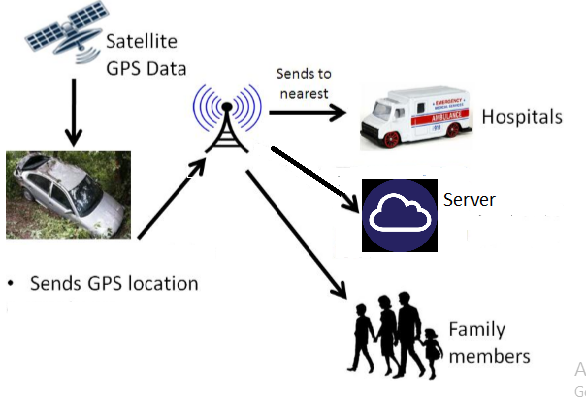
\includegraphics[scale=0.5]{system}
	\caption{System design}
	\label{fig:system}
\end{figure}

The remote server also issues push notifications to other users of the smartphone application.